\documentclass{article}
\usepackage{preamble}

\title{
  \bf\sffamily
  Scalable and Efficient K-Means Data Clustering
}
\author{
  Filemon Mateus \\
  \href{mailto:mateus@utah.edu}{\setfontsize{10}\url{mateus@utah.edu}}
}
\date{}

\begin{document}
  \header{CS 6140 --- Spring 2023}{Data Mining --- Final Project}{\today}
  \maketitle
  \thispagestyle{fancy}

  \begin{abstract}
    This project investigates the performance characteristics of the
    {\sc K-means} clustering algorithm implemented in three distinct
    programming environments: {\sc Python}, {\sc C{\tt ++}}, and {\sc Cuda}.
    The project is aimed at determining the computational efficiency and
    scalability of each computing environment in handling the clustering of
    synthetic multidimensional data points with added Gaussian noise.
    {\sc Python}'s implementation, using libraries such as {\sc SciPy} and
    {\sc ScikitLearn}, focuses on accessibility and ease-of-use. The
    {\sc C{\tt ++}} version leverages low-level control and optimization
    capabilities through the {\sc Standard} and {\sc Eigen} libraries to
    enhance computation speed. Finally, the {\sc Cuda} implementation
    utilizes the parallel processing power of {\sc GPUs} to reduce
    computation times significantly on large datasets. We evaluate the
    execution time, accuracy, and resource utilization of each implementation,
    providing a comprehensive comparison. The insights gained from this
    comparative analysis are crucial for professionals and researchers
    choosing a computing platform for large-scale machine learning tasks.
    This paper aims to serve as a guideline for selecting the appropriate
    programming environment based on specific requirements of computational
    tasks at hand.
  \end{abstract}

  % \tableofcontents

  \section{Repository}
  \begin{itemize}[label={---}]
    \item \url{https://github.com/filemon-mateus/cs6140-final-proj}
  \end{itemize}

  \section{Introduction}
  {\sc K-means} clustering, a cornerstone method in the field of data mining,
  is extensively utilized for its efficiency, interpretability, and simplicity
  in classifying multidimensional datasets into distinct groups \cite{blum2020foundations}.
  As the volume and complexity of data continue to grow, the demand for high-performance
  computing solutions has intensified, prompting a reevaluation of traditional
  approaches to data analysis. Herein, we delve into a comparative
  study of the {\sc K-means} algorithm as implemented in three different
  programming environments: {\sc Python}, {\sc C{\tt ++}}, and {\sc Cuda}. Each
  environment represents a unique approach to computational tasks, with {\sc Python}
  often hailed for its ease of use and integration, {\sc C{\tt ++}} recognized
  for its execution speed and memory control, and {\sc Cuda} acclaimed for its
  capabilities in handling large-scale parallel computations. The primary
  objective of this study is to evaluate and contrast these environments in
  terms of execution efficiency, scalability, and practical usability in data
  clustering tasks. Through a detailed examination of the implementations and
  their performances on synthetic datasets, this paper seeks to provide valuable
  insights into the optimal choices of programming tools based on specific
  use-case scenarios in data analysis and machine learning. This introduction
  sets the stage for a comprehensive analysis of the {\sc K-means} algorithm
  across diverse computing platforms, highlighting the implications of each
  for the field of data mining.

  \section{Background}
  In the clustering problem instance, we are given a training set $X = \{ x^{(1)},
  \ldots, x^{(n)} \}$ of $n$ observations, and want to group $X$ into $k$ cohesive
  ``clusters.'' Here, each entry of $X$, say $x^{(i)}$, is in $\mathbb{R}^d$ as usual;
  but no labels $y^{(i)}$ are given, making this clustering problem instance effectively
  an unsupervised learning problem \cite{ng_k-means}. Solving the closed form algebraic
  representation of the {\sc K-means} algorithm via minimizing the intra-cluster variance
  among the data points is in actuality as hard as solving any other problem in NP
  \cite{phillips2021mathematical}. To circumvent this computational intractability, we
  resort to an iterative approximation algorithm due to Lloyd (1957) which decomposes the
  {\sc K-means} problem into two distinct, alternating steps: the assignment step (found in
  Step 4 of \autoref{alg:kmeans}) and the update step (found in Step 7 of \autoref{alg:kmeans})
  \cite{leskovec2014mining}.

  \begin{algorithm}[H]
    \caption{{\sc K-means}(\{$x^{(1)}, \ldots, x^{(n)}\}, k$)}
    \label{alg:kmeans}
    \begin{algorithmic}[1]
      \State
        Initialized {\bf cluster centroids} $\mu_1, \mu_2, \ldots, \mu_k \in
        \mathbb{R}^d$ randomly.
      \Repeat
        \For{$i \gets 1$ \textbf{to}\ $n$}
          \State $c^{(i)} \gets \displaystyle\arg\min_{j} || x^{(i)} - \mu_j ||^2$.
          \Comment{Assigning Step}
        \EndFor
        \For{$j \gets 1$ \textbf{to}\ $k$}
          \State $\mu_j \gets \displaystyle\frac{\sum_{i=1}^n \mathbbm{1}\{c^{(i)}
          = j\}x^{(i)}}{\sum_{i=1}^n \mathbbm{1}\{c^{(i)} = j\}}$
          \Comment{Updating Step}
        \EndFor
      \Until{{\sc convergence}}
    \end{algorithmic}
  \end{algorithm}

  In the algorithm above, $k$ (a parameter of the algorithm) is number of clusters
  we want to find; and the cluster centroid $\mu_j$ represent our current guesses
  for the positions of the centers of the clusters. To initialize the cluster
  centroids in Step 1 of \autoref{alg:kmeans}, we choose $k$ independent training
  examples at random, and set the cluster centroids to be equal to the values of
  these $k$ examples. The outer-loop of the algorithm repeatedly carries out the
  two steps discussed above: (1) ``assigning'' each training example $x^{(i)}$ to
  the closest cluster centroid $\mu_j$, and (2) moving each cluster centroid $\mu_j$
  to the mean of the points assigned to it.\footnote{
    Outline weakly adapted from: \url{https://cs229.stanford.edu/notes2020spring/cs229-notes7a.pdf}.
  } \medskip

  The convergence in Step 9 of \autoref{alg:kmeans} is affected by the initial
  selection of the centroids in Step 1, which is  often addressed by multiple
  random initializations or by sophisticated methods like the kmeans{\tt ++}
  algorithm, which probabilistically chooses initial centroids to improve cluster
  quality. The computational complexity of {\sc K-means} is generally $O(nkdt)$,
  where $n$ is number of points, $k$ is number of clusters, $d$ is the dimensionality
  of each data point, and $t$ is the number of iterations required for convergence. 
  \medskip

  For the purpose of this paper, we note that parallelization of the {\sc K-means}
  algorithm enhances its performance significantly, making it feasible to handle
  vast and complex datasets that are typical in modern data-driven industries.
  The technique involves dividing the dataset into smaller chunks that can be
  processed concurrently across multiple computing cores or nodes. Each node computes
  the centroids of the clusters for its assigned data segment, and these partial
  results are then aggregated to update the global centroids. This process reduces
  the overall computational burden and leads to faster convergence times. GPU-based
  implementations, particularly using {\sc Cuda}, exploit the massive parallelism of modern
  GPUs, allowing thousands of threads to operate in parallel to perform calculations
  and update centroids in a fraction of the time required by single-threaded solutions.
  This parallel approach not only accelerates the computation but also scales efficiently
  with increasing data sizes and cluster complexities as we will see the next sections.

  \section{Dataset}
  In this project, we plan to generate synthetic datasets from well matured ML libraries
  such as \href{https://scikit-learn.org/}{\url{scikit-learn}} using subroutines like
  {\tt sklearn.datasets.make\_blobs}, which allows for the creation of multi-dimensional
  datasets with controllable numbers of clusters (and centers) and samples. This method
  ensures controlled complexity and reproducibility, which are all essential for systematic
  benchmarking. Furthermore, these synthetic datasets enable precise evaluation of clustering
  algorithms across performance metrics such as speed, scalability, and accuracy since
  the true, ground-truth cluster assignments are known. Additionally, they allow for
  algorithm tuning and optimization in response to varied data characteristics such as
  cluster separation and density, all while avoiding the privacy concerns associated with
  real-world data. Finally, synthetic datasets not only provides flexibility in adjusting
  the complexity and size of the data but also enables the benchmarking of clustering
  performance across different programming paradigms ({\sc Python, C{\tt ++}, Cuda}) and
  dataset scales. In fact, this choice in data acquisition will allow a (possibly useful)
  controlled environment to systematically assess the algorithm's performance across different
  cluster distributions and configurations; thereby, ensuring repeatability and comparability
  of results, crucial for a rigorous benchmark analysis.

  \section{Results}
  \begin{figure}[H]
    \centering
    \begin{subfigure}[b]{0.32\linewidth}
      \centering
      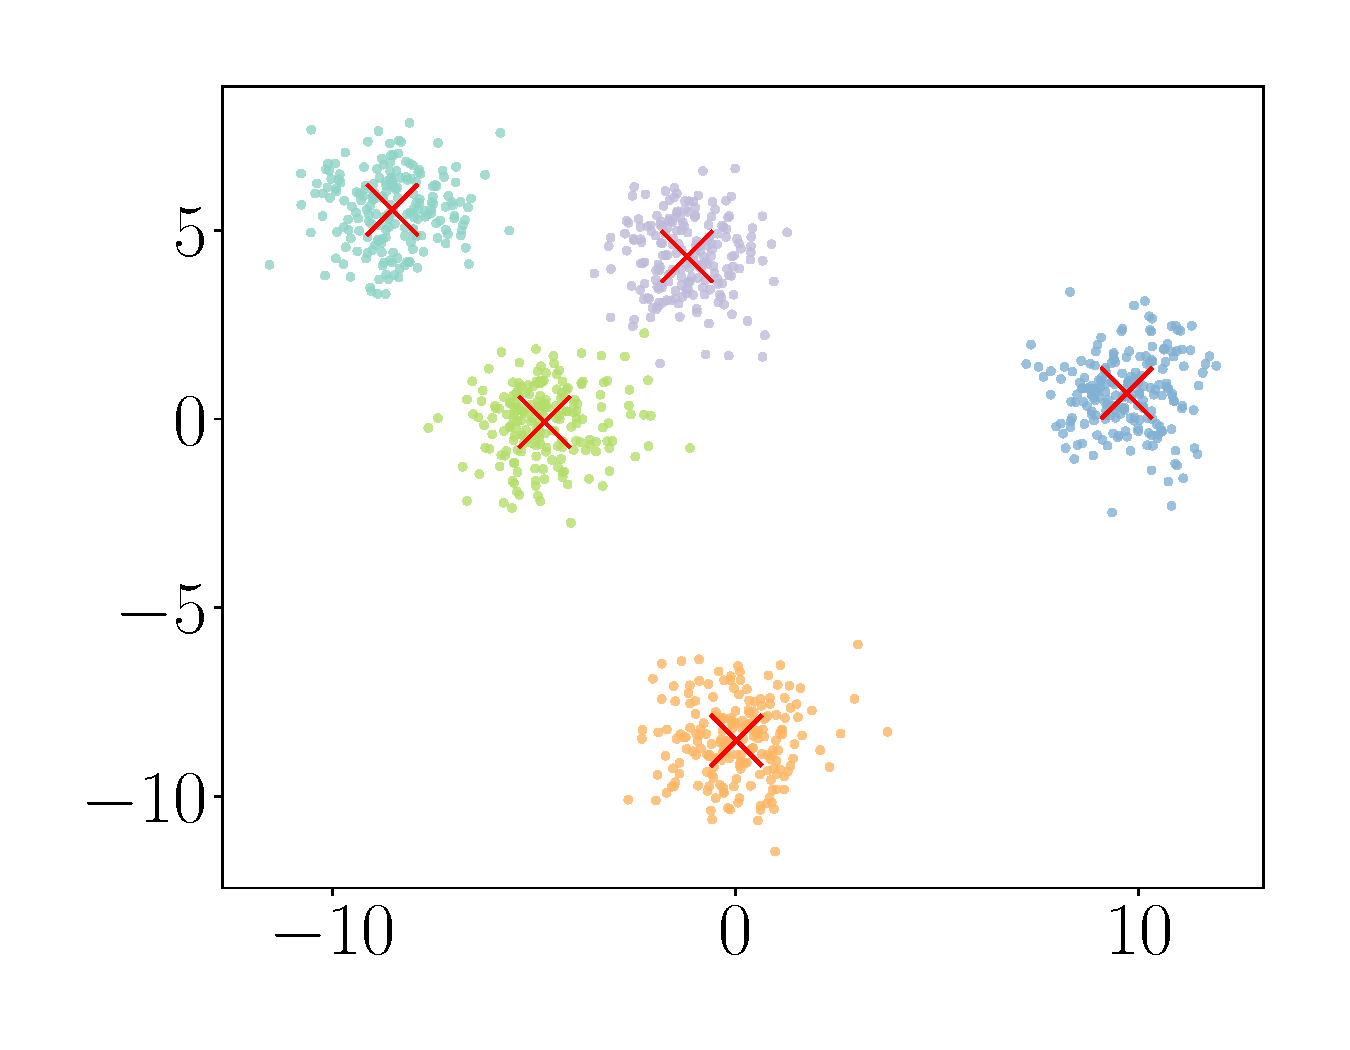
\includegraphics[scale=0.25]{figures/sklpy1K.pdf}
      \caption{\sc Scikit-Learn}
    \end{subfigure}
    \begin{subfigure}[b]{0.32\linewidth}
      \centering
      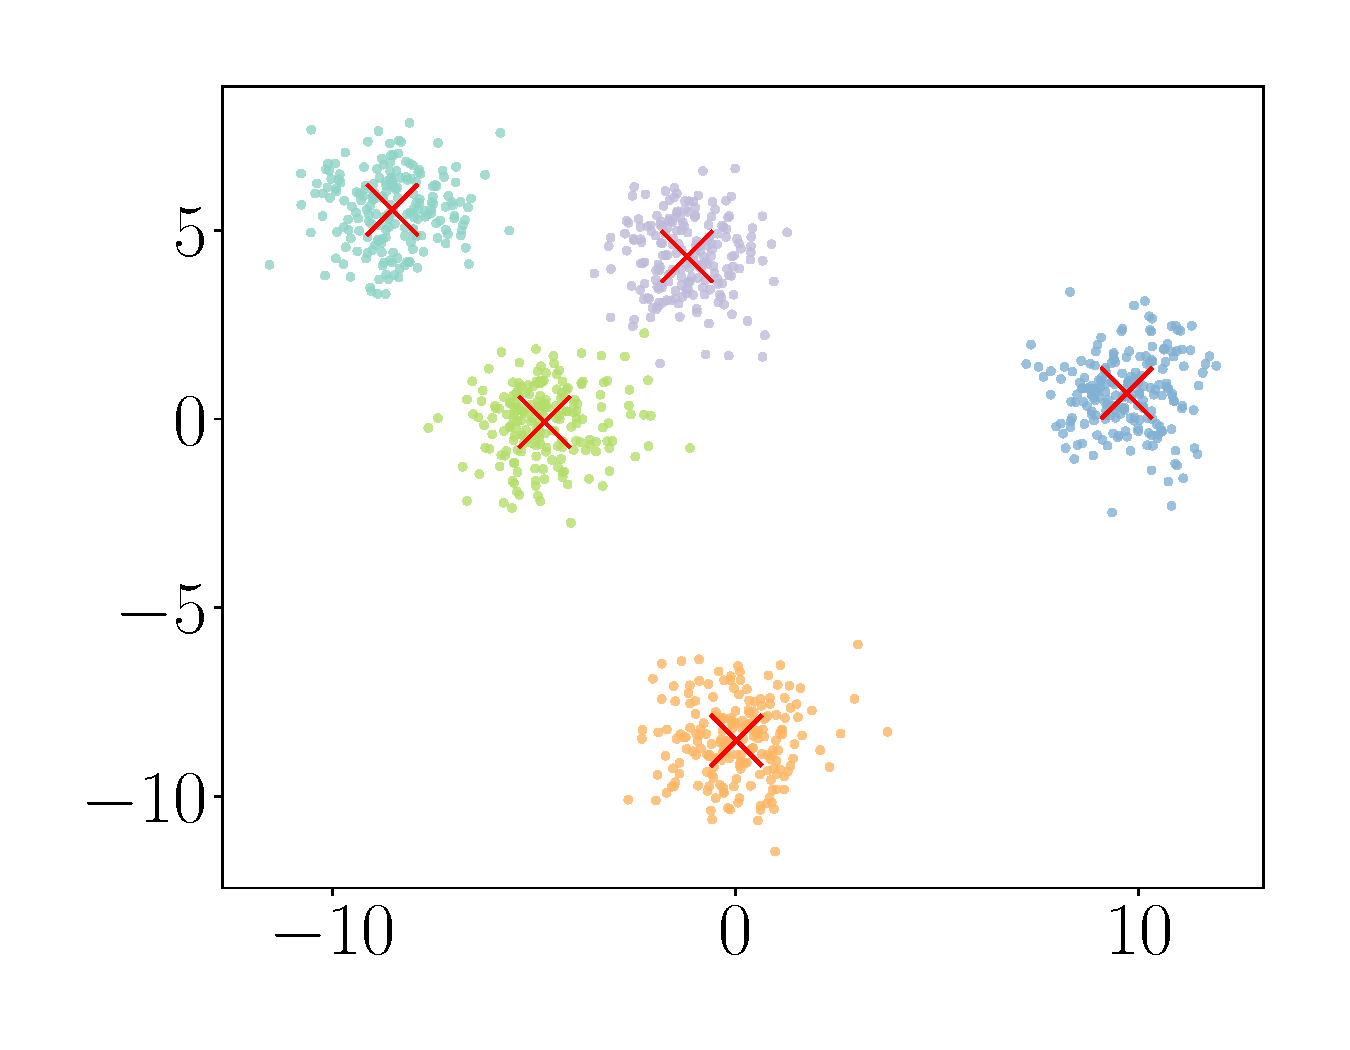
\includegraphics[scale=0.25]{figures/scipy1K.pdf}
      \caption{\sc SciPy}
    \end{subfigure}
    \begin{subfigure}[b]{0.32\linewidth}
      \centering
      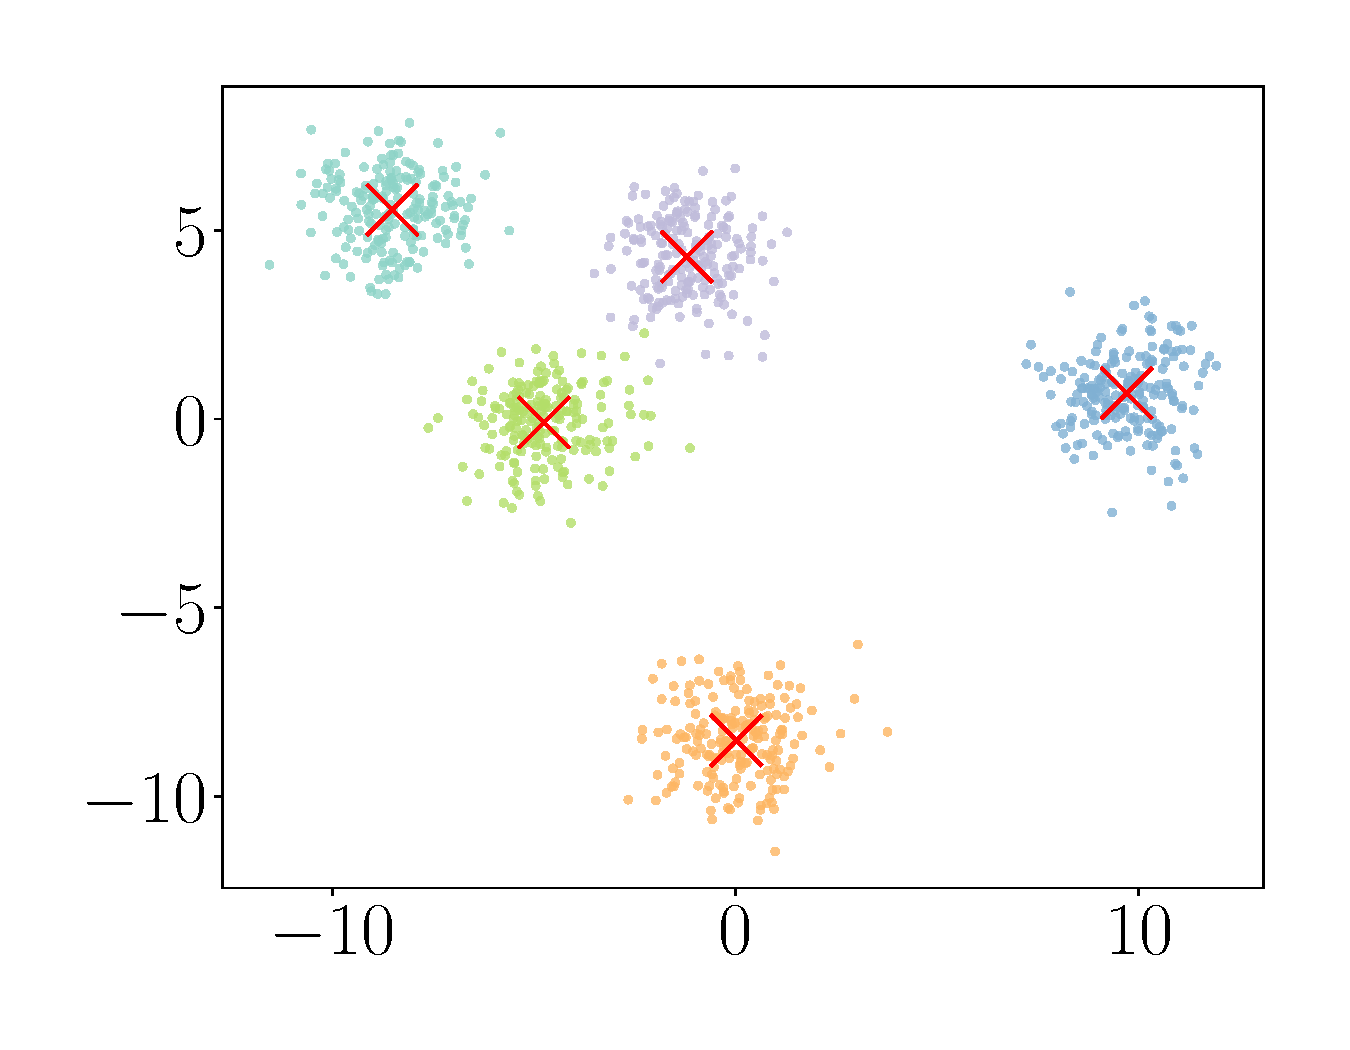
\includegraphics[scale=0.25]{figures/vnlpy1K.pdf}
      \caption{\sc Vanilla Python}
    \end{subfigure}
    \begin{subfigure}[b]{0.32\linewidth}
      \centering
      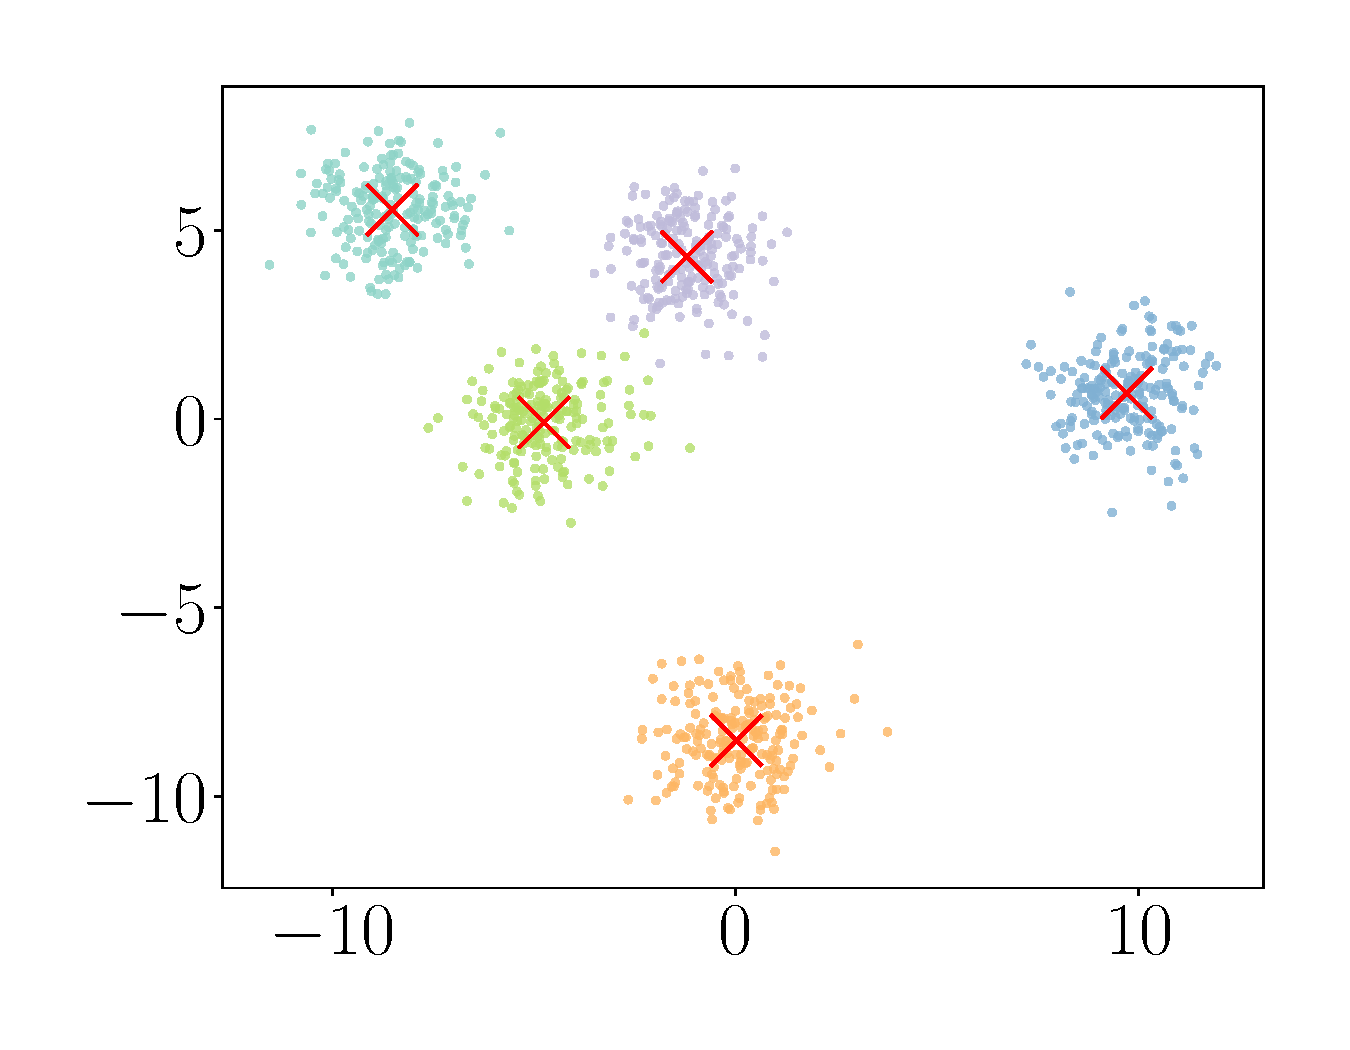
\includegraphics[scale=0.25]{figures/vnlcc1K.pdf}
      \caption{\sc Vanilla C{\tt++} Standard}
    \end{subfigure}
    \begin{subfigure}[b]{0.32\linewidth}
      \centering
      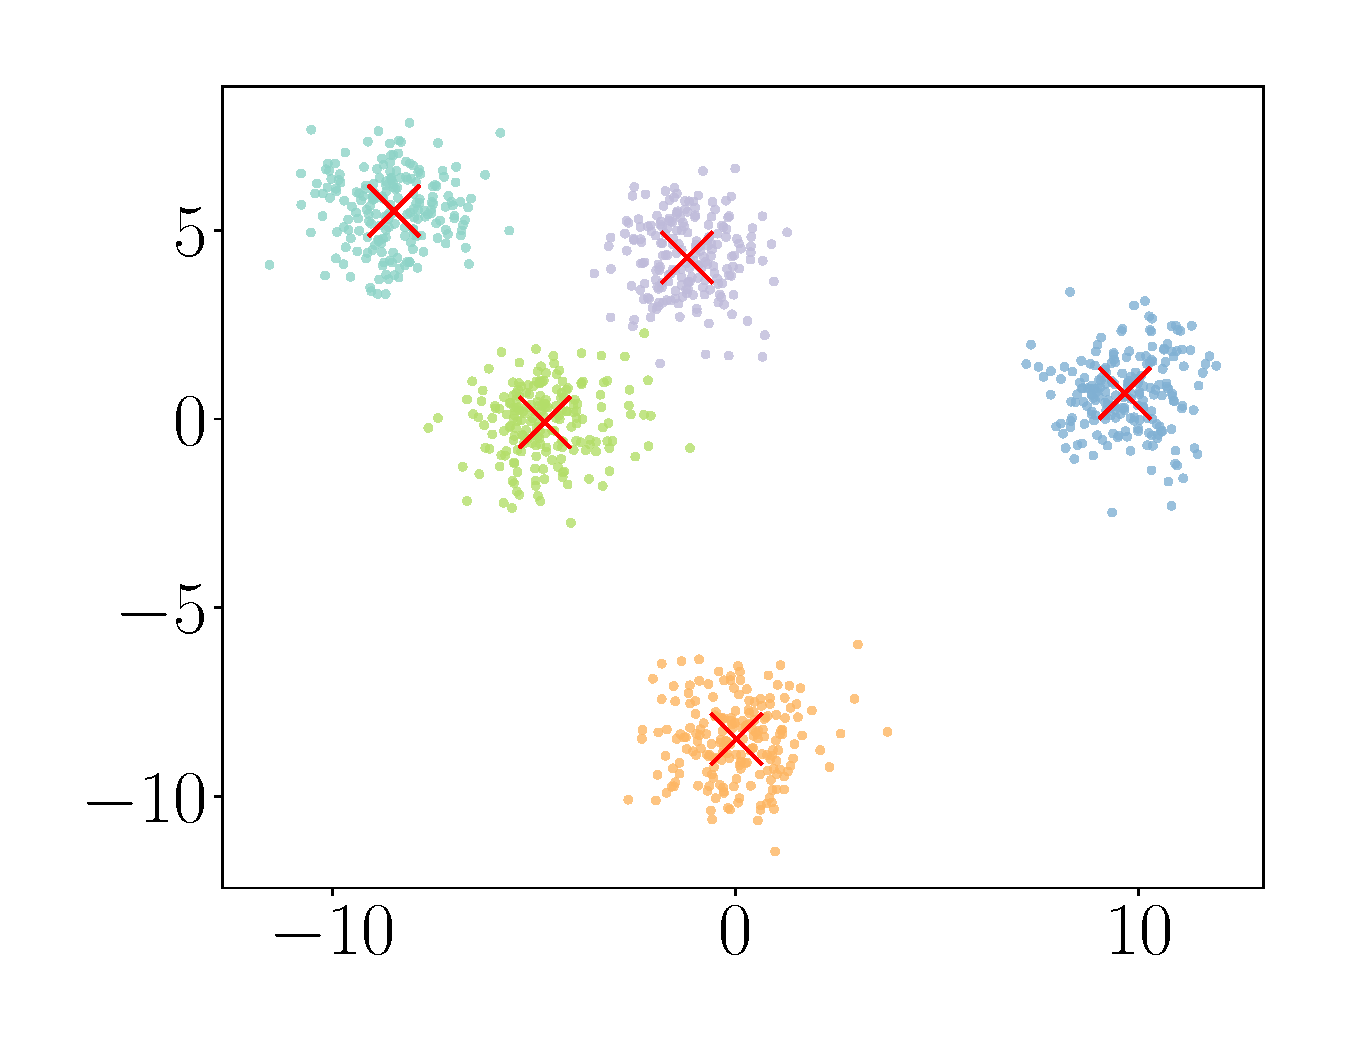
\includegraphics[scale=0.25]{figures/eigcc1K.pdf}
      \caption{\sc Vanilla C{\tt++} Eigen}
    \end{subfigure}
    \begin{subfigure}[b]{0.32\linewidth}
      \centering
      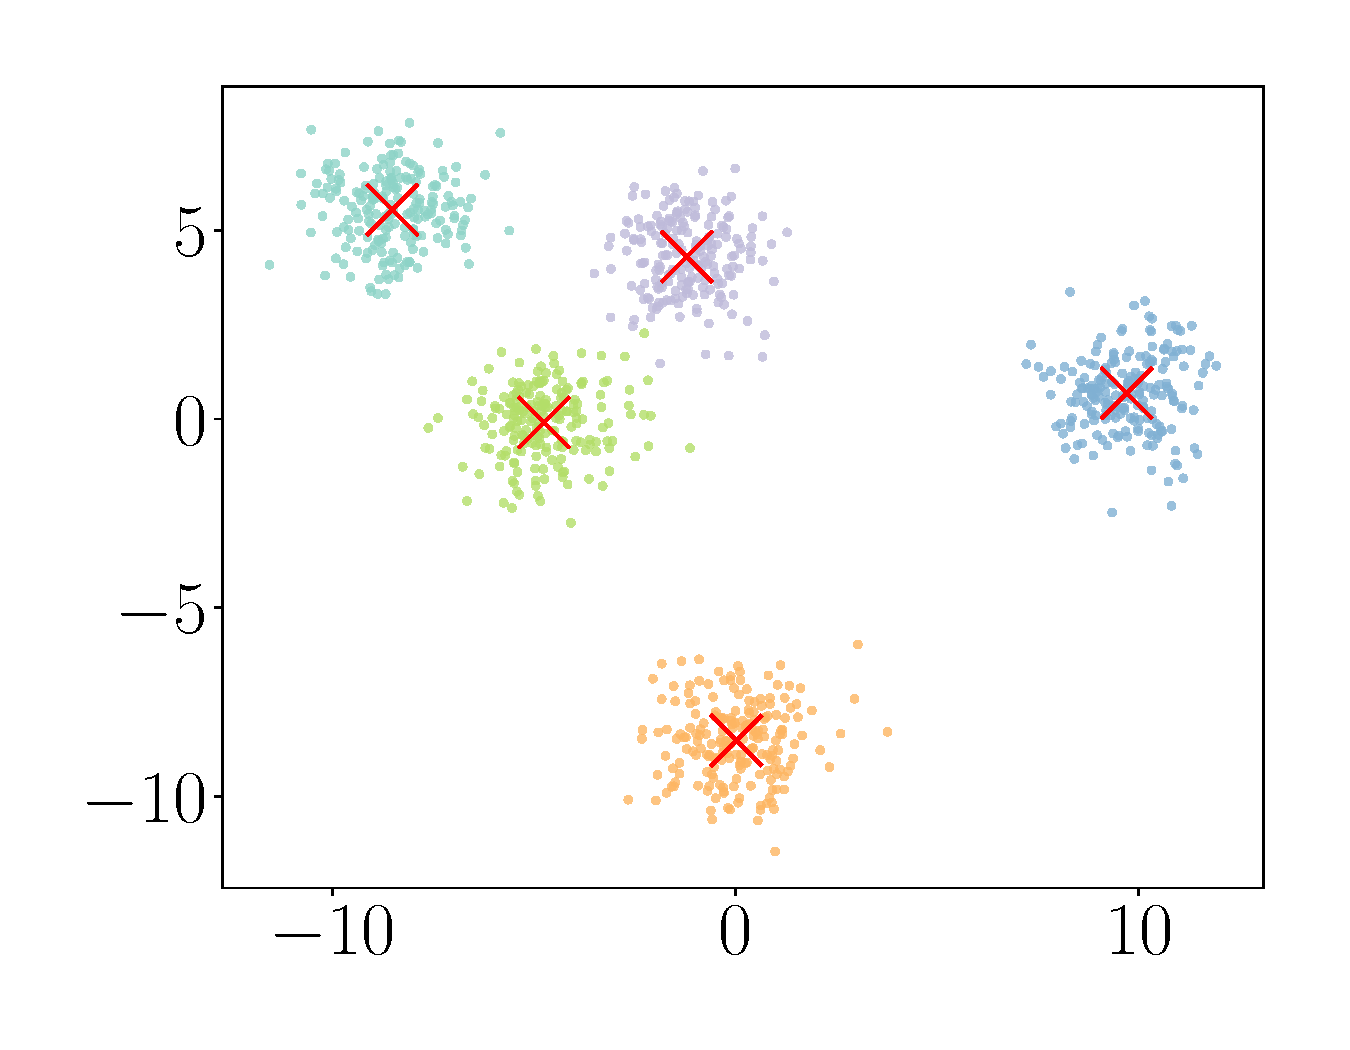
\includegraphics[scale=0.25]{figures/gpu1cc1K.pdf}
      \caption{\sc Cuda v1}
    \end{subfigure}
    \begin{subfigure}[b]{0.32\linewidth}
      \centering
      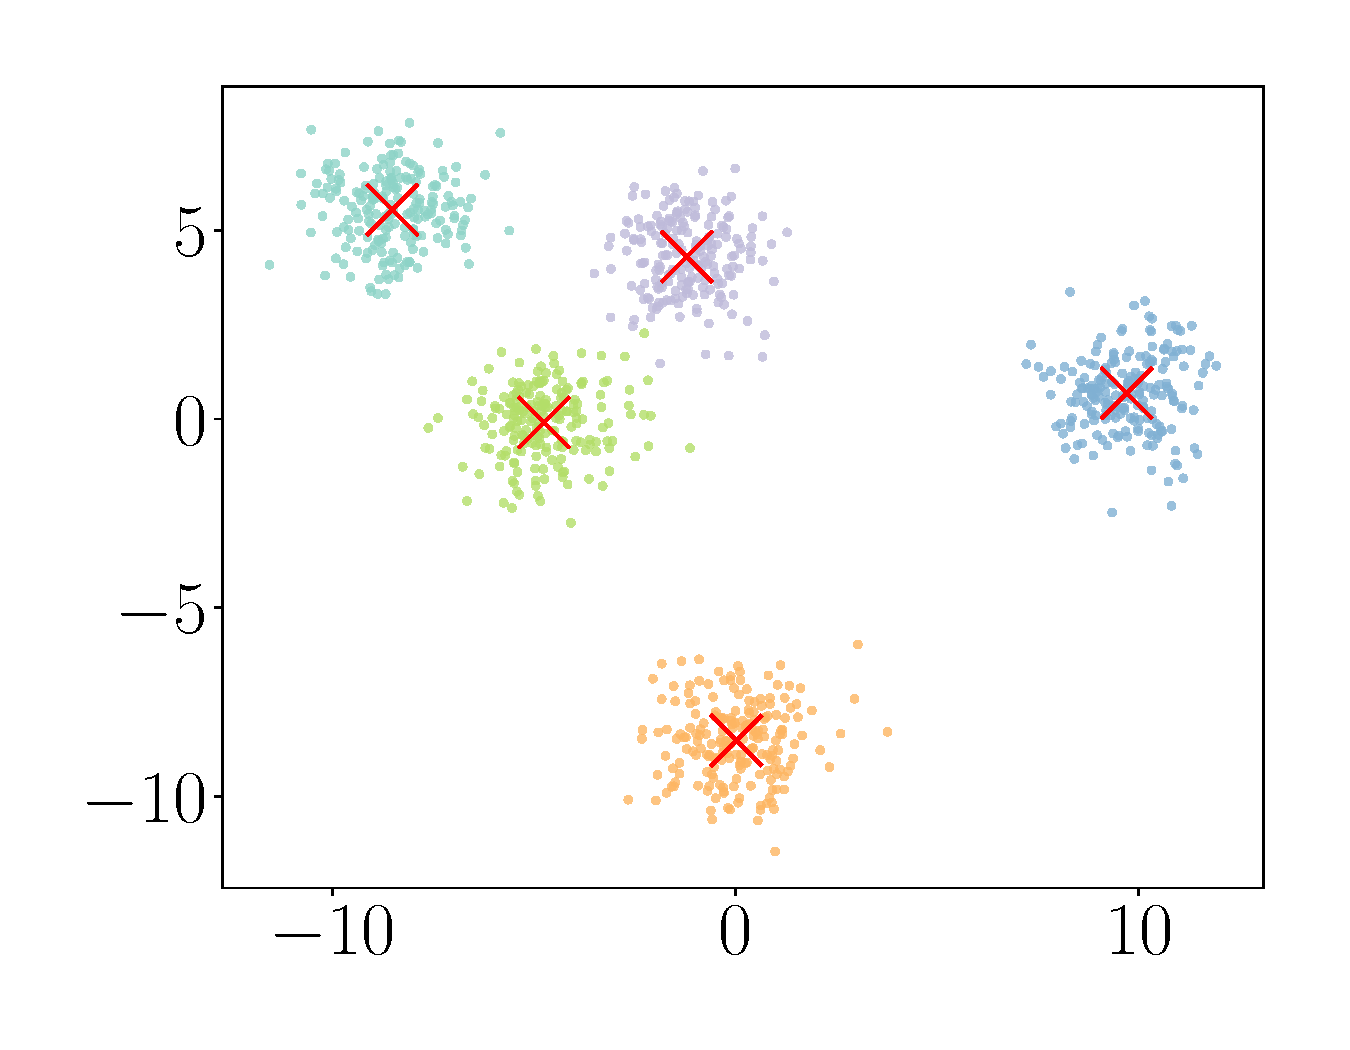
\includegraphics[scale=0.25]{figures/gpu2cc1K.pdf}
      \caption{\sc Cuda v2}
    \end{subfigure}
    \caption{Different implementations of {\sc K-means} algorithm on {\sf 1K.txt} dataset.}
  \end{figure}

  \section{Benchmark}
  \begin{table}[H]
    \centering
    \begin{tabular}{|P{4cm}|P{2.5cm}|P{2.5cm}|P{2.5cm}|P{2.5cm}|P{2.5cm}|}
      \hline
      {\sf Algo/Lib} & {\sf 1K.txt} & {\sf 10K.txt} & {\sf 100K.txt} & {\sf 1M.txt} \\ \hline
      {\sc Scikit-Learn} & {\bf 0.003521} & 0.034318 & 0.535300 & 8.836155 \\
      {\sc SciPy} & 0.027732 & 0.166335 & 1.474478 & 14.327702 \\
      {\sc Vanilla Python} & 0.101650 & 1.221879 & 20.48854 & 191.42883 \\
      {\sc Vanilla C{\tt++} std} & 0.008865 & 0.032988 & 0.254328 & 2.671155 \\
      {\sc Vanilla C{\tt++} eigen} & 0.008202 & 0.034422 & 0.294001 & 3.425298 \\
      {\sc Cuda v1} & 0.009314 & 0.041698 & 0.090047 & 0.652350 \\
      {\sc Cuda v2} & 0.006274 & {\bf 0.029613} & {\bf 0.053129} & {\bf 0.215813} \\ \hline
    \end{tabular}
    \caption{
      Runtime Benchmark --- this table shows the runtime performance measured in
      seconds of different {\sc K-means} implementations across various data sizes,
      highlighting how GPU-accelerated versions ({\sc Cuda v1} and {\sc Cuda v2})
      dramatically reduce computation times, especially in larger datasets, compared
      to CPU-based implementations ({\sc Scikit-Learn}, {\sc SciPy}, {\sc Vanilla
      Python}, {\sc Vanilla C{\tt++} standard}, and {\sc Vanilla C{\tt++} eigen}).
    }
    \label{tbl:runtime}
  \end{table}

  Pictorially, \autoref{tbl:runtime} translates to the following plot:
  \begin{figure}[H]
    \centering
    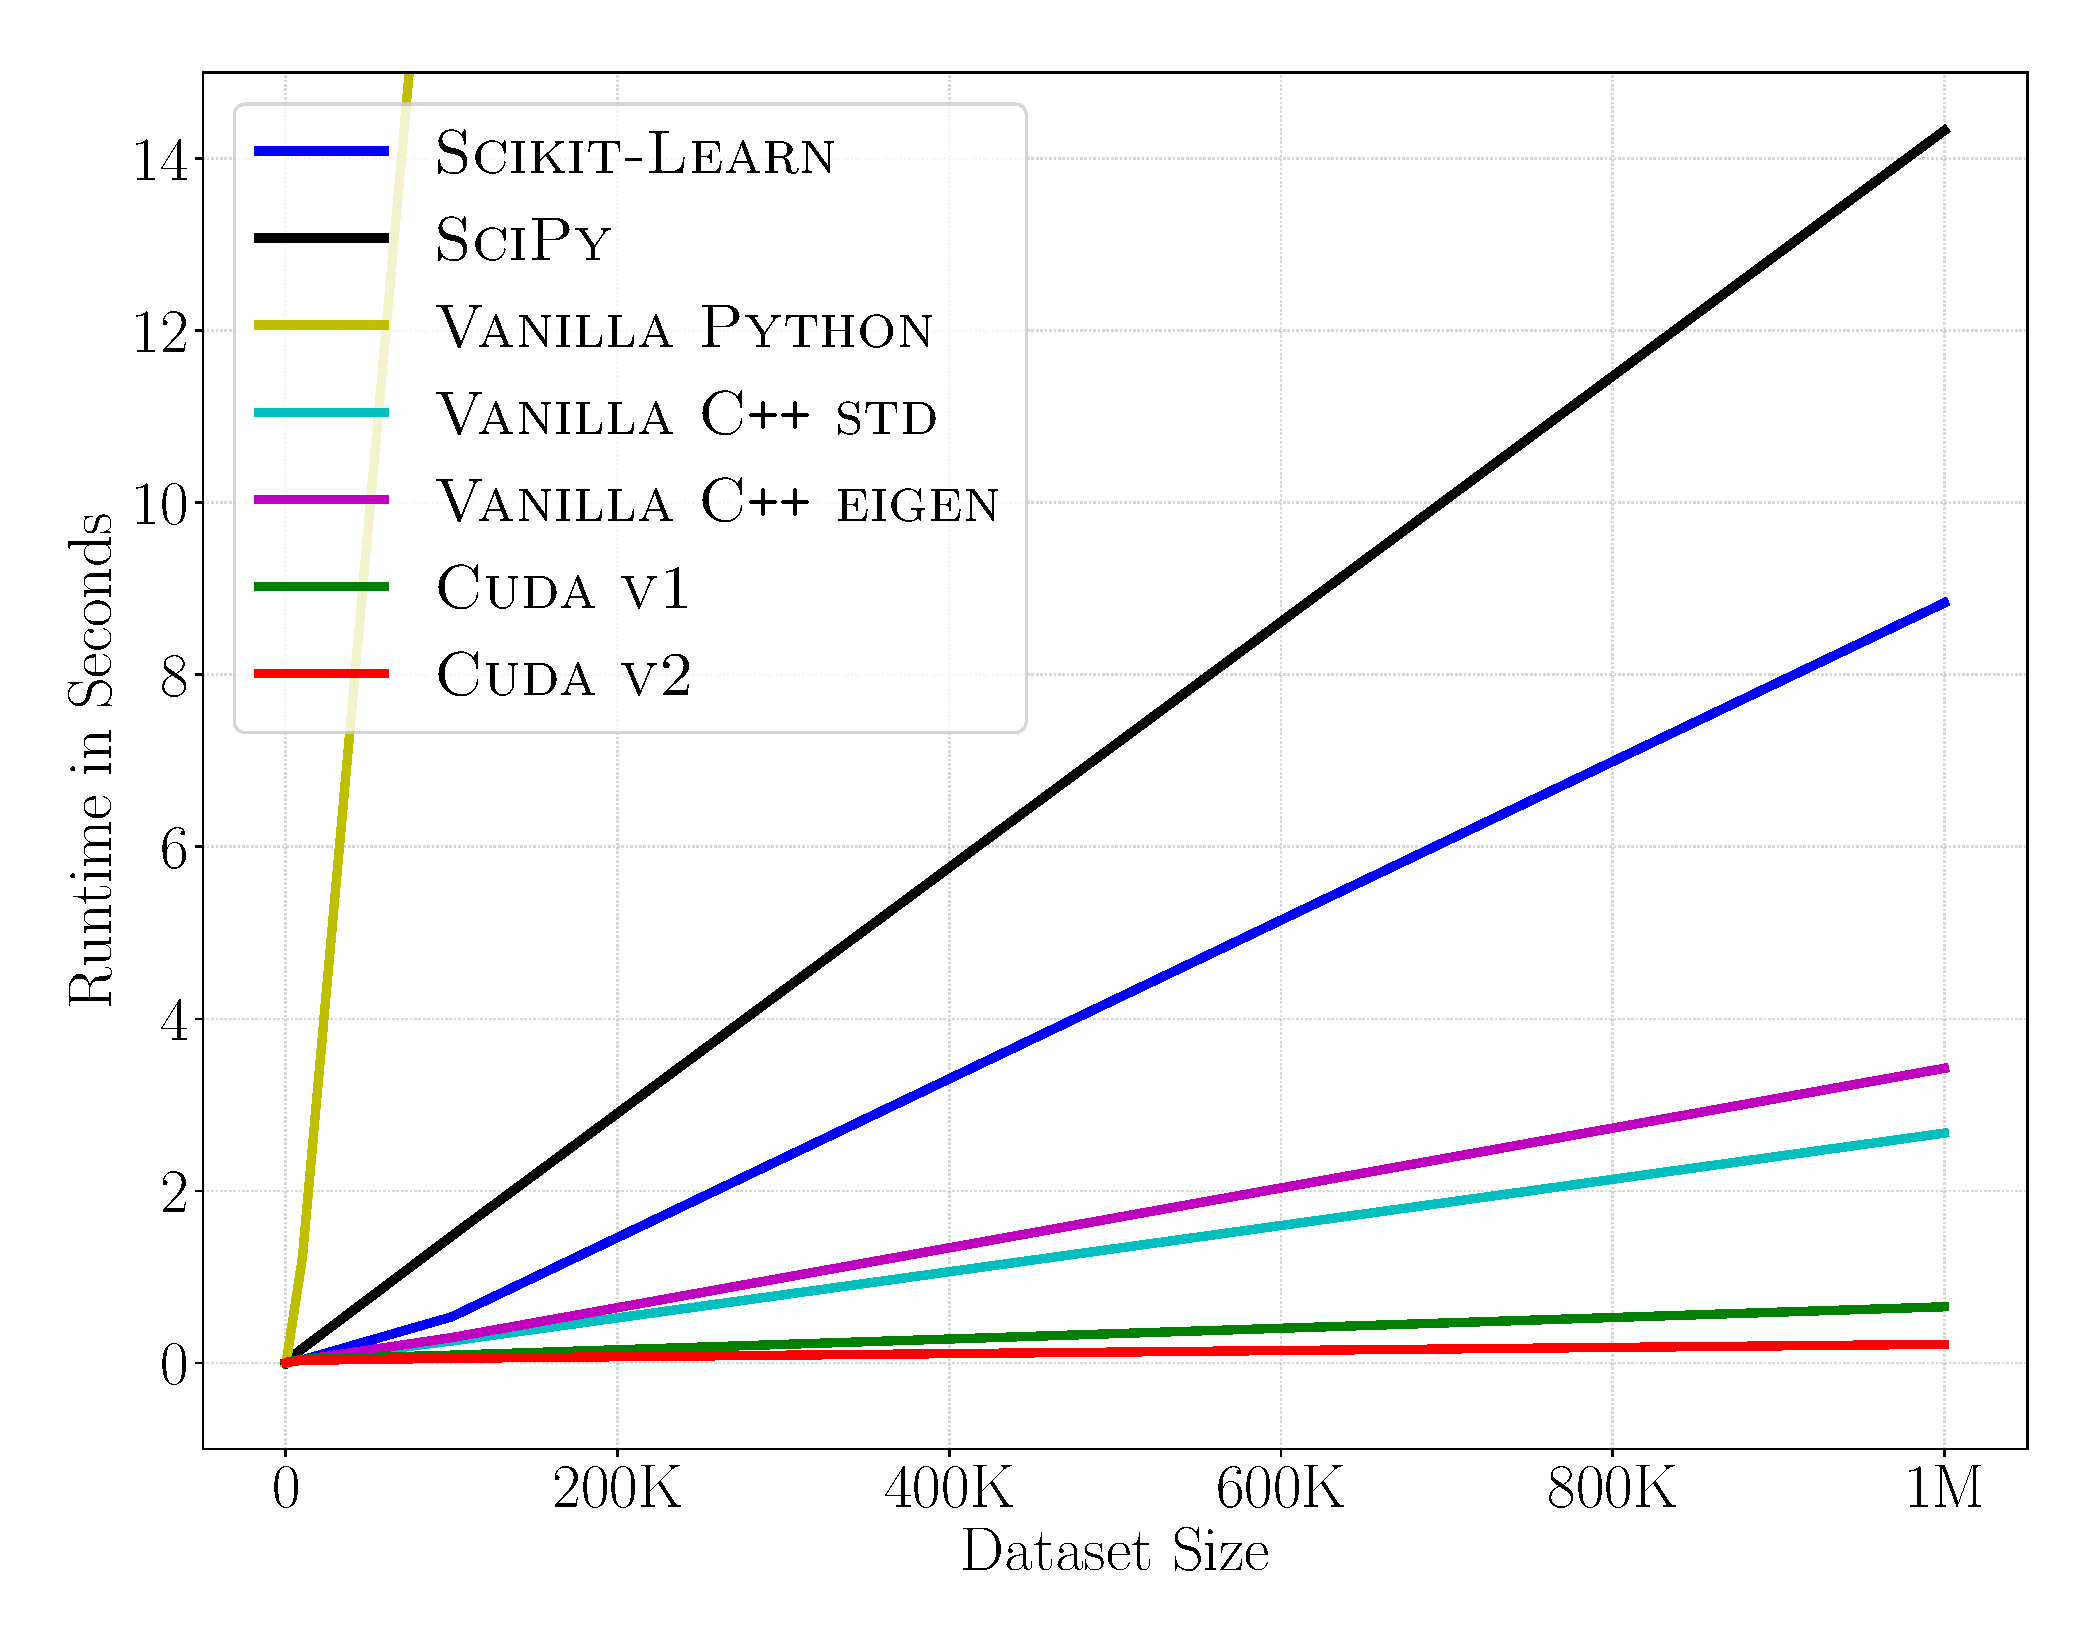
\includegraphics[scale=0.25]{figures/runtime.pdf}
    \caption{Runtime Benchmark.}
    \label{fig:runtime}
  \end{figure}

  \begin{table}[H]
    \centering
    \begin{tabular}{|P{4cm}|P{2.5cm}|P{2.5cm}|P{2.5cm}|P{2.5cm}|P{2.5cm}|}
      \hline
      {\sf Algo/Lib} & {\sf 1K.txt} & {\sf 10K.txt} & {\sf 100K.txt} & {\sf 1M.txt} \\ \hline
      {\sc Scikit-Learn} & 0.756701 & 0.756096 & 0.749256 & 0.754255 \\
      {\sc SciPy} & 0.756701 & 0.752882 & 0.752448 & 0.752540 \\
      {\sc Vanilla Python} & 0.756701 & 0.759022 & 0.749302 & 0.752429 \\
      {\sc Vanilla C{\tt++} std} & 0.756701 & 0.752345 & 0.752440 & 0.745546 \\
      {\sc Vanilla C{\tt++} eigen} & 0.756701 & 0.756139 & 0.747363 & 0.755571 \\
      {\sc Cuda v1} & 0.756701 & 0.753208 & 0.755416 & 0.746047 \\
      {\sc Cuda v2} & 0.756701 & 0.753208 & 0.755416 & 0.746047 \\ \hline
    \end{tabular}
    \caption{
      Silhouette Score of the Mean Silhouette Coefficient of all Samples --- this
      table presents the silhouette scores for each implementation across different
      dataset sizes, illustrating generally consistent clustering quality across
      all implementations with slight variation as the dataset size increases from
      left to right.
    }
    \label{tbl:silhouette}
  \end{table}

  Pictorially, \autoref{tbl:silhouette} translates to the following plot:
  \begin{figure}[H]
    \centering
    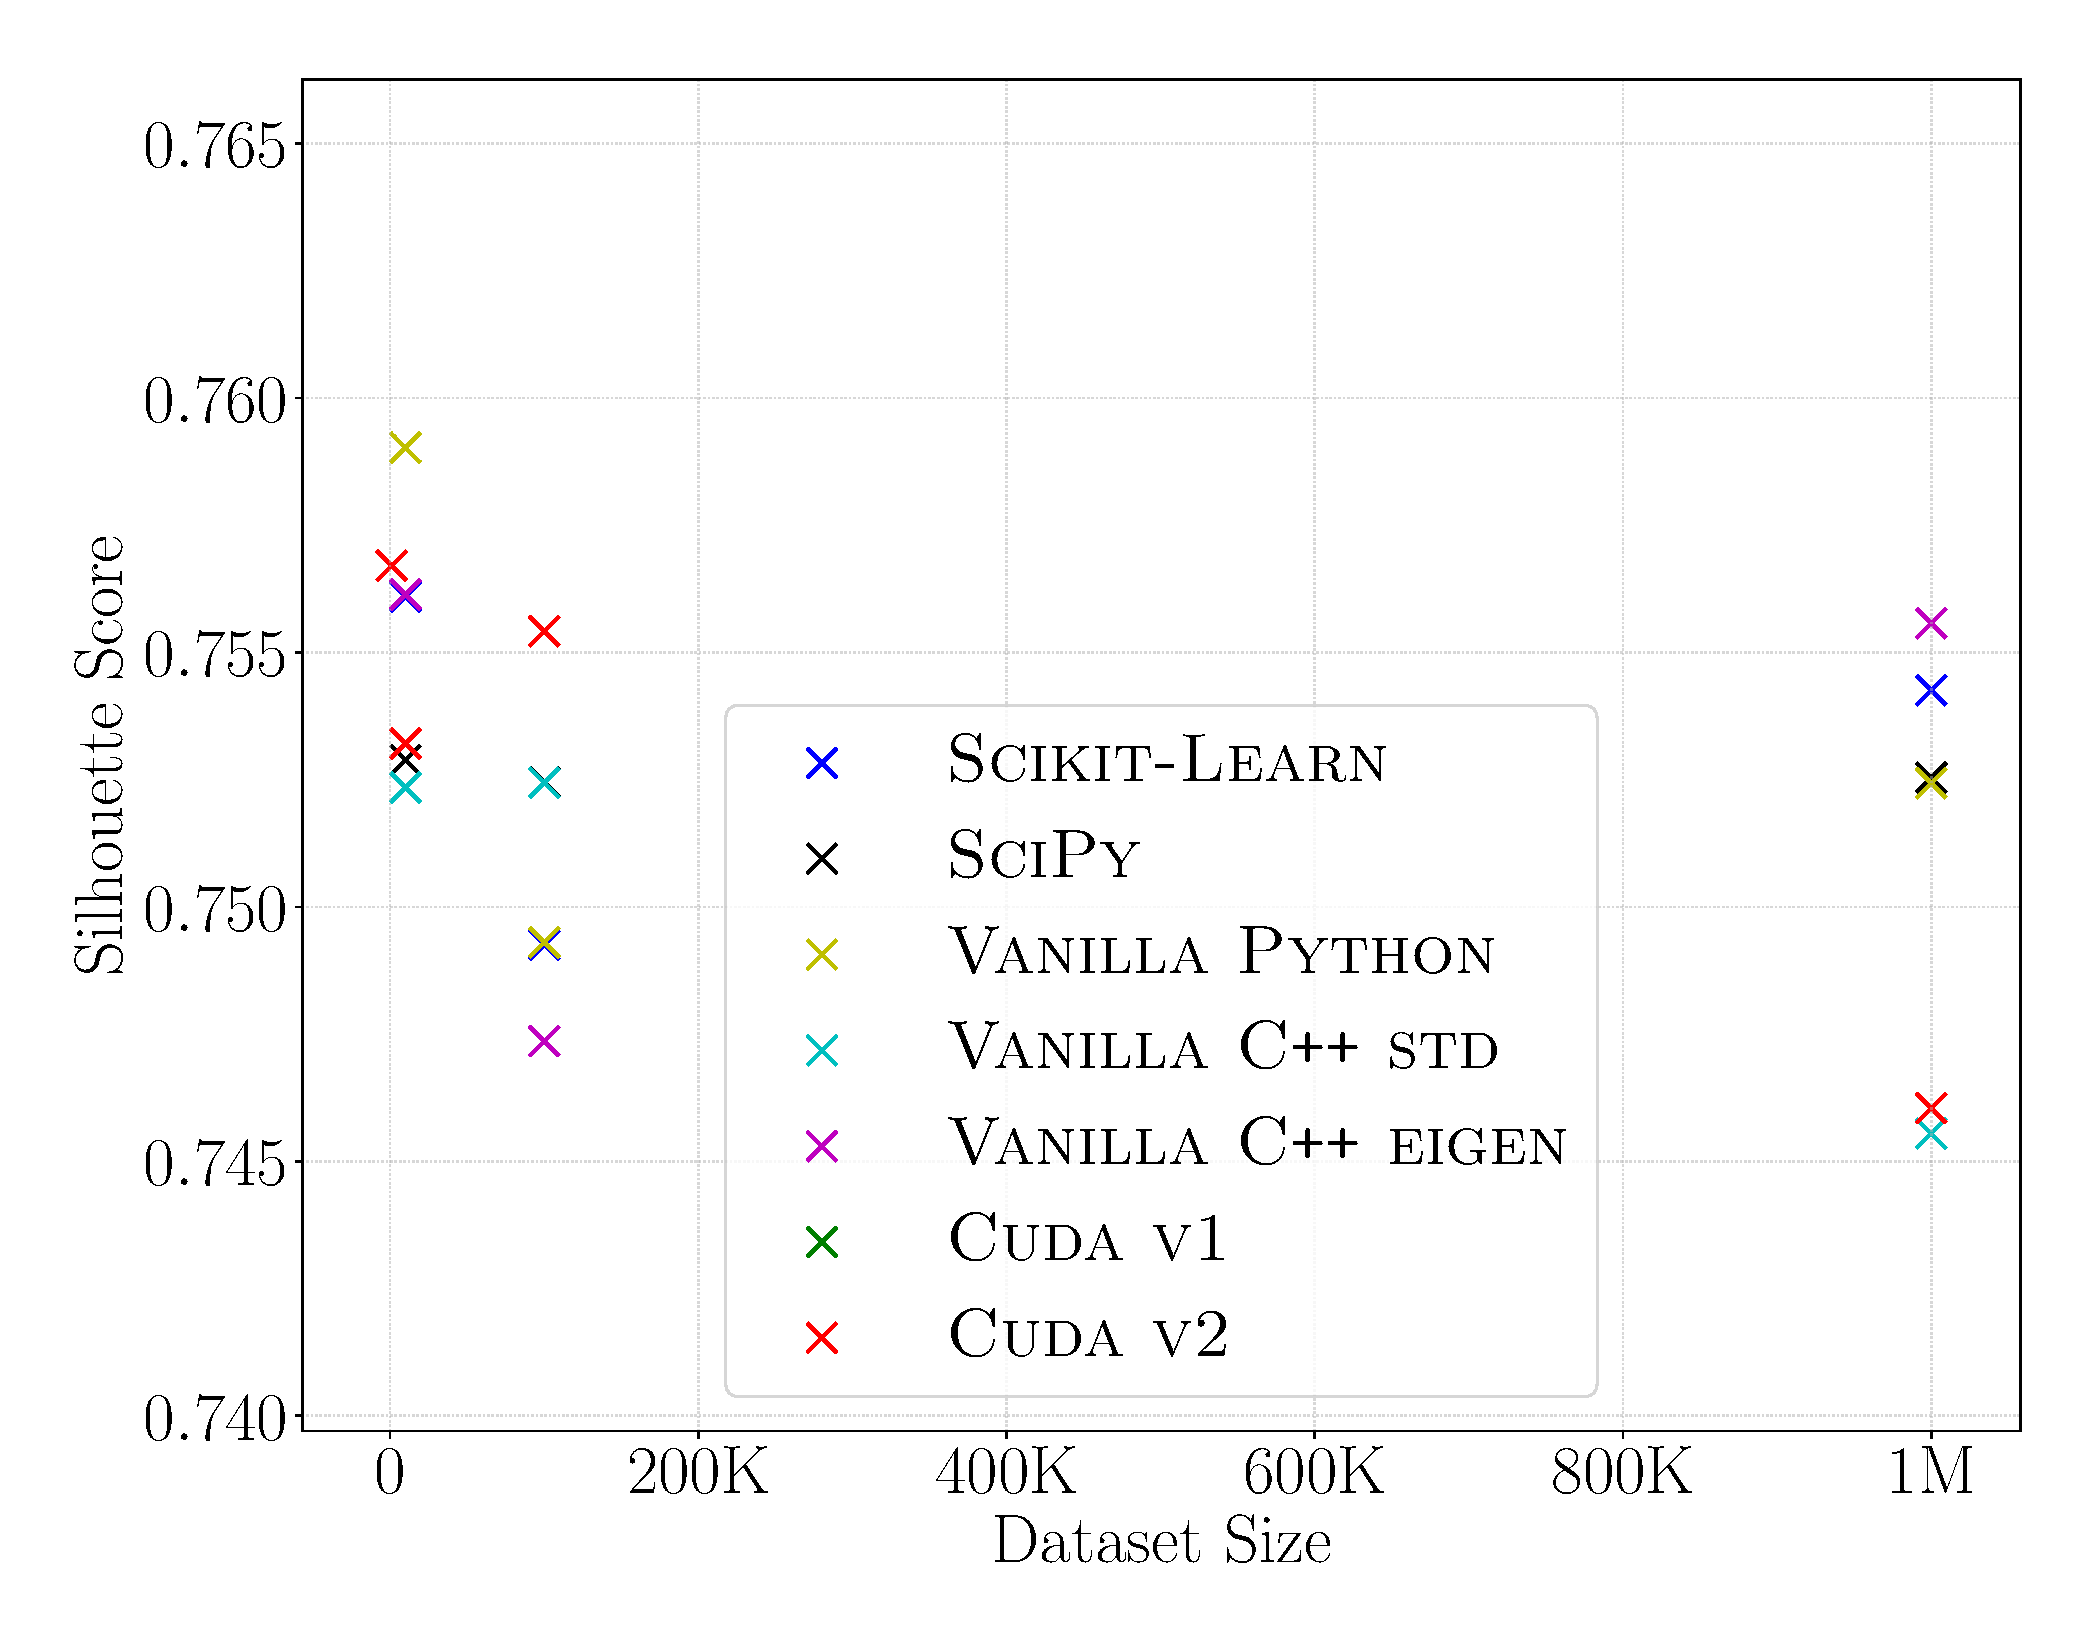
\includegraphics[scale=0.25]{figures/silhouette.pdf}
    \caption{Silhouette Scores.}
  \end{figure}

  \begin{table}[H]
    \centering
    \begin{tabular}{|P{4cm}|P{2.5cm}|P{2.5cm}|P{2.5cm}|P{2.5cm}|P{2.5cm}|}
      \hline
      {\sf Algo/Lib} & {\sf 1K.txt} & {\sf 10K.txt} & {\sf 100K.txt} & {\sf 1M.txt} \\ \hline
      {\sc Scikit-Learn} & 0.996065 & 0.993236 & 0.994860 & 0.994549 \\
      {\sc SciPy} & 0.996065 & 0.993236 & 0.994860 & 0.994549 \\
      {\sc Vanilla Python} & 0.996065 & 0.993236 & 0.994860 & 0.994549 \\
      {\sc Vanilla C{\tt++} std} & 0.996065 & 0.993236 & 0.994860 & 0.994549 \\
      {\sc Vanilla C{\tt++} eigen} & 0.996065 & 0.993236 & 0.994860 & 0.994549 \\
      {\sc Cuda v1} & 0.996065 & 0.993236 & 0.994860 & 0.994549 \\
      {\sc Cuda v2} & 0.996065 & 0.993236 & 0.994860 & 0.994549 \\ \hline
    \end{tabular}
    \caption{
      Adjusted Mutual Score (i.e. Accuracy Permutation Independent Score) --- this
      table displays the adjusted mutual scores for each implementation, and confirms
      the accuracy and consistency of clustering results across different programming
      environments, indicating high similarity in cluster assignments regardless of
      the underlying computational approach.
    }
    \label{tbl:accuracy}
  \end{table}

  \begin{table}[H]
    \centering
    \begin{tabular}{|P{4cm}|P{2.5cm}|P{2.5cm}|P{2.5cm}|P{2.5cm}|P{2.5cm}|}
      \hline
      {\sf Algo/Lib} & {\sf 1K.txt} & {\sf 10K.txt} & {\sf 100K.txt} & {\sf 1M.txt} \\ \hline
      {\sc Scikit-Learn} & 1.390736 & 1.397050 & 1.410765 & 1.413165 \\
      {\sc SciPy} & 1.390736 & 1.397050 & 1.410765 & 1.413165 \\
      {\sc Vanilla Python} & 1.390706 & 1.397045 & 1.410765 & 1.413165 \\
      {\sc Vanilla C{\tt++} std} & 1.390706 & 1.397045 & 1.410765 & 1.413165 \\
      {\sc Vanilla C{\tt++} eigen} & 1.391263 & 1.397050 & 1.410765 & 1.413165 \\
      {\sc Cuda v1} & 1.390706 & 1.397045 & 1.410765 & 1.413165 \\
      {\sc Cuda v2} & 1.390706 & 1.397045 & 1.410765 & 1.413165 \\ \hline
    \end{tabular}
    \caption{
      $k$-means cost --- this table provides the k-means cost for each implementation
      and dataset size, showing uniform costs across all methods, which implies
      consistent performance in terms of clustering efficiency.
    }
    \label{tbl:kmeans-cost}
  \end{table}

  \begin{table}[H]
    \centering
    \begin{tabular}{|P{4cm}|P{2.5cm}|P{2.5cm}|P{2.5cm}|P{2.5cm}|P{2.5cm}|}
      \hline
      {\sf Algo/Lib} & {\sf 1K.txt} & {\sf 10K.txt} & {\sf 100K.txt} & {\sf 1M.txt} \\ \hline
      {\sc Scikit-Learn} & 3.940704 & 4.167821 & 4.924603 & 5.492129 \\
      {\sc SciPy} & 3.940704 & 4.167821 & 4.924603 & 5.492129 \\
      {\sc Vanilla Python} & 3.940704 & 4.167821 & 4.924530 & 5.491405 \\
      {\sc Vanilla C{\tt++} std} & 3.940705 & 4.167809 & 4.924526 & 5.491415 \\
      {\sc Vanilla C{\tt++} eigen} & 3.913538 & 4.163677 & 4.924756 & 5.491409 \\
      {\sc Cuda v1} & 3.940705 & 4.167809 & 4.924526 & 5.491415 \\
      {\sc Cuda v2} & 3.940705 & 4.167809 & 4.924526 & 5.491415 \\ \hline
    \end{tabular}
    \caption{
      $k$-center cost --- listing the $k$-center costs for each {\sc K-means}
      implementation, this table reveals identical costs across all environments,
      suggesting that the centroid positioning is effectively consistent among
      different implementations.
    }
    \label{tbl:kcenter-cost}
  \end{table}

  \begin{table}[H]
    \centering
    \begin{tabular}{|P{4cm}|P{2.5cm}|P{2.5cm}|P{2.5cm}|P{2.5cm}|P{2.5cm}|}
      \hline
      {\sf Algo/Lib} & {\sf 1K.txt} & {\sf 10K.txt} & {\sf 100K.txt} & {\sf 1M.txt} \\ \hline
      {\sc Scikit-Learn} & 1.234888 & 1.238547 & 1.250711 & 1.252577 \\
      {\sc SciPy} & 1.234888 & 1.238547 & 1.250711 & 1.252577 \\
      {\sc Vanilla Python} & 1.234840 & 1.238538 & 1.250713 & 1.252577 \\
      {\sc Vanilla C{\tt++} std} & 1.234840 & 1.238538 & 1.250713 & 1.252577 \\
      {\sc Vanilla C{\tt++} eigen} & 1.235289 & 1.238534 & 1.250712 & 1.252577 \\
      {\sc Cuda v1} & 1.234840 & 1.238538 & 1.250713 & 1.252577 \\
      {\sc Cuda v2} & 1.234840 & 1.238538 & 1.250713 & 1.252577 \\ \hline
    \end{tabular}
    \caption{
      $k$-medians cost --- the results for $k$-medians cost from this table
      shows nearly the same for all implementations across various dataset
      sizes, highlighting a uniform distribution of medians in the clustering
      results produced by each implementation environment.
    }
    \label{tbl:kmedians-cost}
  \end{table}

  From the benchmarks, it is evident that all {\sc K-means} implementations produce
  identically the same clusters with nearly identical adjusted mutual scores (see
  \autoref{tbl:accuracy}), silhouette scores (see \autoref{tbl:silhouette}), kmeans
  cost (see \autoref{tbl:kmeans-cost}), kcenter cost (see \autoref{tbl:kcenter-cost}),
  and kmedians cost (see \autoref{tbl:kmedians-cost}). The contrast, however, rests
  on the runtime taken to produce these clusters, where we see a distinct difference
  in the runtime performance of the {\sc K-means} implementations across  various
  programming environments and datasets sizes. \medskip

  Starting with {\sc Python} implementations, {\sc Scikit-Learn} demonstrates highly
  efficient runtime characteristics, especially noticeable in smaller datasets.
  For example, its runtime is merely {\bf 0.003521} seconds for the {\sf 1K.txt} dataset,
  scaling up to {\bf 8.836155} seconds for the {\sf 1M.txt} dataset. {\sc SciPy}
  show less optimized performance compared to {\sc Scikit-Learn}, starting from
  {\bf 0.027732} seconds and going up to {\bf 14.327702} seconds for the same dataset
  sizes, indicating a slightly higher computational overhead. \medskip

  The {\sc Vanilla Python} implementation, unsurprisingly, shows the least efficiency
  among the {\sc Python} variants, with a dramatic increase in runtime as dataset
  size grows (from {\bf 0.101650} seconds to a staggering {\bf 191.423883} seconds),
  reflecting the lack for low-level optimizations and reliance on pure {\sc Python}'s
  slower execution speed. \medskip

  In contrast, the {\sc C{\tt ++}} implementation offer significant runtime reductions.
  Both {\sc Vanilla C{\tt++} standard} and {\sc Vanilla C{\tt++} eigen} start at
  approximately {\bf 0.008} seconds for the {\sf 1K.txt} dataset and remain under
  {\bf 4} seconds even for the {\sf 1M.txt} dataset. This is indicative of the
  effectiveness of C{\tt++}'s low-level optimizations and memory management capabilities,
  which provide additional computational efficiency for matrix operations and numerical
  solvers. \medskip

  The {\sc Cuda} implementations show exceptional runtime performance by exploiting
  {\sc GPU} parallelism. {\sc Cuda v1} starts at {\bf 0.009341} seconds for the
  {\sf 1K.txt} dataset and scales up to {\bf 0.0652350} seconds for the {\sf 1M.txt}
  dataset. {\sc Cuda v2}, an even more optimized version which uses a logarithmic
  tree-reduction on its shared memory (see \autoref{lst:kmeans-gpu2}), begins
  {\bf 0.006274} and ends at {\bf 0.215813} seconds for the {\sf 1M.txt} dataset,
  showcasing the substantial benefits of fine-tuned GPU computations in handling
  large-scale data efficiently. \medskip

  These runtime performances are graphically represented in \autoref{fig:runtime},
  where we can visually assess the scalability and efficiency of each implementation
  as datasets size increases. This comparison highlights the substantial runtime
  performance gains that can be attained through more sophisticated programming
  environments and the use of specific computational techniques like GPU acceleration
  in {\sc Cuda}. Such insights are crucial for choosing the right computing platform
  based on the specific needs of large-scale data mining tasks, where both data
  size and computational efficiency are critical factors.

  \section{Discussion}
  In this comparative study of {\sc K-means} implementations across various programming
  environments, the performance metrics clearly favor the {\sc CUDA v2} implementation
  on GPUS. This implementation not only excels in handling large datasets but also
  drastically reduces computational times when compared to more traditional CPU-based
  approaches like {\sc Scikit-Learn} and {\sc SciPy}. \medskip

  Specifically, {\sc Cuda v2} outperforms {\sc Scikit-Learn} by up to {\bf 41 times}
  and surpasses {\sc SciPy} by up to {\bf 66 times} on the {\sf 1M.txt} dataset. Such a
  stark difference in performance underscores the significant advantage of utilizing
  GPU-based parallel processing over CPU-based methods, particularly for task involving
  large volumes of data. \medskip

  The superior performance of {\sc CUDA v2} can be attributed to its ability to leverage
  the massive parallelism of modern GPUs. This allows thousands of threads to operate
  simultaneously, significantly speeding up the computation and updating of centroids,
  which are crucial operations in the {\sc K-means} algorithm. This capability not only
  provides a boost in speed but also enhances scalability, making it a suitable choice
  for real-world applications that require handling of big data efficiently. \medskip

  However, while {\sc Cuda v2} presents substantial benefits in terms of speed and
  scalability, it necessitates specific hardware and expertise in parallel programming,
  which may not be readily available in all settings. In contrast, {\sc Scikit-Learn}
  and {\sc SciPy}, while slower, offer greater accessibility and ease of use, with
  extensive support and documentation that can be advantageous for novice users with
  less technical expertise or computational resources. \medskip

  In conclusion, the choice between these environments should be guided by the specific
  requirements of the task, including dataset size, computational resources, and available
  expertise. For large-scale applications where time efficiency is paramount, and appropriate
  hardware is available, {\sc Cuda v2} is clearly the superior contender. Conversely, for
  smaller projects or environments where simplicity and accessibility are more critical,
  {\sc Scikit-Learn} or {\sc SciPy} might be more appropriate despite their slower
  performance.

  \printbibliography[heading=bibnumbered]

  \newpage

  \section{Appendix}
  \subsection{\sc Scikit-Learn}
  \lstinputlisting
    [
      caption={\sf kmeans-skl.py},
      firstline=56,
      lastline=77
    ]
    {../kmeans-skl1.py}

  \subsection{\sc SciPy}
  \lstinputlisting
    [
      caption={\sf kmeans-sci.py},
      firstline=56,
      lastline=77
    ]
    {../kmeans-sci1.py}

  \subsection{\sc Vanilla Python}
  \lstinputlisting
    [
      caption={\sf kmeans-vnl.py},
      firstline=47,
      lastline=65
    ]
    {../kmeans-vnl1.py}

  \subsection{\sc Vanilla C{\tt++} standard}
  \lstinputlisting
    [
      caption={\sf kmeans-vnl.cc},
      firstline=31,
      lastline=72
    ]
    {../kmeans-vnl1.cc}

  \subsection{\sc Vanilla C{\tt++} eigen}
  \lstinputlisting
    [
      caption={\sf kmeans-eig.cc},
      firstline=16,
      lastline=46
    ]
    {../kmeans-eig1.cc}

  \subsection{\sc Cuda v1}
  \lstinputlisting
    [
      caption={\sf kmeans-gpu1.cu},
      firstline=48,
      lastline=91
    ]
    {../kmeans-gpu1.cu}

  \subsection{\sc Cuda v2}
  \lstinputlisting
    [
      caption={\sf kmeans-gpu2.cu},
      label={lst:kmeans-gpu2},
      firstline=46,
      lastline=152
    ]
    {../kmeans-gpu2.cu}
\end{document}
